% Options for packages loaded elsewhere
\PassOptionsToPackage{unicode}{hyperref}
\PassOptionsToPackage{hyphens}{url}
\documentclass[
]{article}
\usepackage{xcolor}
\usepackage{amsmath,amssymb}
\setcounter{secnumdepth}{-\maxdimen} % remove section numbering
\usepackage{iftex}
\ifPDFTeX
  \usepackage[T1]{fontenc}
  \usepackage[utf8]{inputenc}
  \usepackage{textcomp} % provide euro and other symbols
\else % if luatex or xetex
  \usepackage{unicode-math} % this also loads fontspec
  \defaultfontfeatures{Scale=MatchLowercase}
  \defaultfontfeatures[\rmfamily]{Ligatures=TeX,Scale=1}
\fi
\usepackage{lmodern}
\ifPDFTeX\else
  % xetex/luatex font selection
\fi
% Use upquote if available, for straight quotes in verbatim environments
\IfFileExists{upquote.sty}{\usepackage{upquote}}{}
\IfFileExists{microtype.sty}{% use microtype if available
  \usepackage[]{microtype}
  \UseMicrotypeSet[protrusion]{basicmath} % disable protrusion for tt fonts
}{}
\makeatletter
\@ifundefined{KOMAClassName}{% if non-KOMA class
  \IfFileExists{parskip.sty}{%
    \usepackage{parskip}
  }{% else
    \setlength{\parindent}{0pt}
    \setlength{\parskip}{6pt plus 2pt minus 1pt}}
}{% if KOMA class
  \KOMAoptions{parskip=half}}
\makeatother
\usepackage{longtable,booktabs,array}
\newcounter{none} % for unnumbered tables
\usepackage{calc} % for calculating minipage widths
% Correct order of tables after \paragraph or \subparagraph
\usepackage{etoolbox}
\makeatletter
\patchcmd\longtable{\par}{\if@noskipsec\mbox{}\fi\par}{}{}
\makeatother
% Allow footnotes in longtable head/foot
\IfFileExists{footnotehyper.sty}{\usepackage{footnotehyper}}{\usepackage{footnote}}
\makesavenoteenv{longtable}
\usepackage{graphicx}
\makeatletter
\newsavebox\pandoc@box
\newcommand*\pandocbounded[1]{% scales image to fit in text height/width
  \sbox\pandoc@box{#1}%
  \Gscale@div\@tempa{\textheight}{\dimexpr\ht\pandoc@box+\dp\pandoc@box\relax}%
  \Gscale@div\@tempb{\linewidth}{\wd\pandoc@box}%
  \ifdim\@tempb\p@<\@tempa\p@\let\@tempa\@tempb\fi% select the smaller of both
  \ifdim\@tempa\p@<\p@\scalebox{\@tempa}{\usebox\pandoc@box}%
  \else\usebox{\pandoc@box}%
  \fi%
}
% Set default figure placement to htbp
\def\fps@figure{htbp}
\makeatother
\setlength{\emergencystretch}{3em} % prevent overfull lines
\providecommand{\tightlist}{%
  \setlength{\itemsep}{0pt}\setlength{\parskip}{0pt}}
\usepackage{bookmark}
\IfFileExists{xurl.sty}{\usepackage{xurl}}{} % add URL line breaks if available
\urlstyle{same}
\hypersetup{
  hidelinks,
  pdfcreator={LaTeX via pandoc}}

\author{}
\date{}

\begin{document}

\section{Paper 7: Configuration Statistics and Relational
Readout}\label{paper-7-configuration-statistics-and-relational-readout}

\subsection{Derivation of Exclusion Statistics, the Stable-Species
Spectrum, Timeless Branching Ratios, and the Birth of Relational
Geometry with Its Holographic
Readout}\label{derivation-of-exclusion-statistics-the-stable-species-spectrum-timeless-branching-ratios-and-the-birth-of-relational-geometry-with-its-holographic-readout}

Author: Noriaki Kihara\\
Affiliation: WF System Co., Ltd.\\
ORCID: 0009-0004-6753-4020\\
Version: v0.2\\
Date: June 2026\\
DOI (this version): 10.5281/zenodo.20640459\\
Concept DOI: 10.5281/zenodo.20640458\\
License: CC BY 4.0

\begin{center}\rule{0.5\linewidth}{0.5pt}\end{center}

\subsection{Abstract}\label{abstract}

This paper introduces a \textbf{configuration reading} into the
reciprocal dual model (Papers 1--6): the fragments after splitting are
occupied cells of a shared parent lattice, and a state is the
\textbf{set} of occupied cells. From this minimal embedding hypothesis,
the following are derived.

First, \textbf{exclusion statistics}: since a state is a set, no label
of ``which fragment is which'' exists, and double occupancy of the same
cell is impossible by the non-overlap = orthogonality theorem (Paper 5).
Indistinguishability and the exclusion principle become theorem-like
consequences, not assumptions.

Second, the \textbf{stable-species spectrum}: from exclusion follows the
shell capacity law \(n_m\le c(m)\), and an exhaustive scan (\(s\le25\))
of the allowed decay channels under odd partitions and the capacity law
establishes that \(s=1,3,5\) are \textbf{absolutely stable} (no channel
exists) and that the decay threshold is \(s=7\). For the first time the
model possesses a spectrum of stable states.

Third, \textbf{timeless branching ratios}: the question ``when, and
triggered by what, does decay occur'' is ill-posed in this model, where
time = a sequence of events; the absence of a trigger (spontaneity) is a
constitutive principle of time. What can be predicted are the relative
weights among channels (branching ratios), and at \(s=9\) the
configuration counting of the two allowed channels yields the unique
ratio \((5,3,1):(3,3,3)=192:56\) (77.4\% : 22.6\%).

Fourth, the \textbf{birth and readout of relational geometry}: the
configuration of a single fragment is a non-observable under the \(B_4\)
gauge, but with two or more fragments, for the first time, the inner
products = angles between occupied cells become gauge invariants. We
show that this relational data can be read out completely from the
\(\lambda\)-side record (the intensity of the interference pattern)
alone: the five relation classes of the \(s=9\) final decay
configurations are completely separated by the multiplicity-weighted
power spectrum alone (a theorem over all 248 configurations), and the
entirety of the data required for identification is obtained exactly
from \textbf{a single unit record} (the unit-record sufficiency
theorem). The amplitudes lie on a discrete alphabet of powers of
\(\sqrt2\), and the readout is digital decoding. Channels containing the
minimal fragment (the zero mode) are of \textbf{holographic type},
permitting complete reconstruction of the configuration; channels
without it are of \textbf{interferometric type}, yielding relations
only.

Finally, as consequences of the exclusion rule, we show that within a
shared lattice the existing occupancy blocks the decay channels of other
fragments --- a \textbf{blocking effect} (environment dependence of
decay channels) --- and that the timeless state space of small systems
can be enumerated completely as a finite closed set.

\begin{center}\rule{0.5\linewidth}{0.5pt}\end{center}

\subsection{Keywords}\label{keywords}

exclusion principle, indistinguishability, configuration space, stable
spectrum, branching ratio, gauge invariant, relational geometry,
holography, digital decoding, selection rule

\begin{center}\rule{0.5\linewidth}{0.5pt}\end{center}

\subsection{1. Introduction}\label{introduction}

The kinematics established in Paper 6 {[}3{]} (the freezing theorem, the
\(B_4\) gauge, and the record theorem) is the preparation for treating
systems in which multiple fragments coexist. This paper asks two
questions:

\begin{enumerate}
\def\labelenumi{\arabic{enumi}.}
\tightlist
\item
  What statistics do multiple fragments obey --- are they
  distinguishable, and can they share the same cell?
\item
  Are the relations among fragments (distances, angles) observables ---
  and if so, from which records can they be read?
\end{enumerate}

Quantum statistics (the Pauli exclusion principle {[}5{]}, Fermi--Dirac
statistics {[}6,7{]}) is introduced in standard theory as an empirical
rule or as a consequence of field quantization. The equal a priori
probability of statistical mechanics is a postulate (for foundational
discussion, see Jaynes {[}8{]}). The viewpoint that only relative
quantities are observable in the absence of a reference frame has been
systematized in the quantum-information context (Bartlett, Rudolph \&
Spekkens {[}9{]}). This paper reconstructs these results \textbf{in a
form exhaustively verifiable within a finite lattice model}: the
statistics are derived from the configuration reading, the equal-weight
rule is made explicit as the counting principle of the model, the
observability of relations only follows from the record theorem (Paper
6), and the concrete readout procedure is given by a mechanism
structurally isomorphic to holography (Gabor {[}10{]}).

\begin{center}\rule{0.5\linewidth}{0.5pt}\end{center}

\subsection{2. The Configuration Reading (Minimal Embedding
Hypothesis)}\label{the-configuration-reading-minimal-embedding-hypothesis}

\begin{quote}
\textbf{Hypothesis (configuration reading)}: The fragments after
splitting are occupied cells of a shared parent lattice. The
representative value of a fragment is the \(r_{\max}(k)^2\) of its
occupied cell, i.e., an energy-like quantity = the radial position
within frequency space. A state = the \textbf{set} of occupied cells.
\end{quote}

All components used are pre-existing: the lattice (Paper 2 {[}4{]}),
representativization (Paper 5 {[}2{]} §6.4), non-overlap = orthogonality
(Paper 5 §5), and binary occupancy. It is a concretization of the
finite-\(R'\) splitting representation of Paper 4 {[}1{]} as occupancy
of a shared parent lattice. It is a minimal construction with zero new
components, but we make explicit that it is a \textbf{choice} of
embedding (independent verification is provided by the readout theorems
of §6).

\subsubsection{2.1 Derivation of exclusion
statistics}\label{derivation-of-exclusion-statistics}

Since a state is a set of occupied cells, (i) fragments carry no
individual labels (a set contains no duplicates), and (ii) double
occupancy of the same cell is impossible by the orthogonality theorem.

\begin{quote}
\textbf{Consequence}: Fragments are indistinguishable occupancies and
obey the exclusion principle. The statistics are not an assumption but a
theorem-like consequence of binary occupancy + orthogonality.
\end{quote}

\begin{center}\rule{0.5\linewidth}{0.5pt}\end{center}

\subsection{3. The Shell Capacity Law and the Stable-Species
Spectrum}\label{the-shell-capacity-law-and-the-stable-species-spectrum}

\subsubsection{3.1 The capacity law}\label{the-capacity-law}

The number of cells in each shell \(m\) is
\(c(m)=1,8,24,40,64,96,96,144,\ldots\) (Paper 5 §8). From exclusion,

\[
n_m\le c(m)
\]

(the number of fragments with label \(m\) is at most the shell
capacity). In particular \(c(1)=1\): \textbf{at most one fragment with
label 1 in the system}.

\subsubsection{3.2 The stable-species
spectrum}\label{the-stable-species-spectrum}

Exhaustive scan of allowed channels under odd partitions (the
consistency condition of Paper 5) + the capacity law:

{\def\LTcaptype{none} % do not increment counter
\begin{longtable}[]{@{}rll@{}}
\toprule\noalign{}
\(s\) & Number of allowed channels & Remark \\
\midrule\noalign{}
\endhead
\bottomrule\noalign{}
\endlastfoot
1, 3, 5 & \textbf{0 (absolutely stable)} & \\
7 & 1 (only (3,3,1)) & decay threshold \\
9 & 2 ((5,3,1), (3,3,3)) & \\
11 & 3 & \\
13 & 5 & includes the smallest 5-body channel \\
25 & 37 & the number of channels grows rapidly with \(s\) \\
\end{longtable}
}

\begin{quote}
\textbf{Main result}: For \(s=1,3,5\) no channel exists kinematically,
so they are absolutely stable. The decay threshold is \(s=7\). The
capacity law eliminates 5 of the naive 7 channels at \(s=9\) (those
containing multiple \(s=1\), etc.).
\end{quote}

\begin{figure}
\centering
\pandocbounded{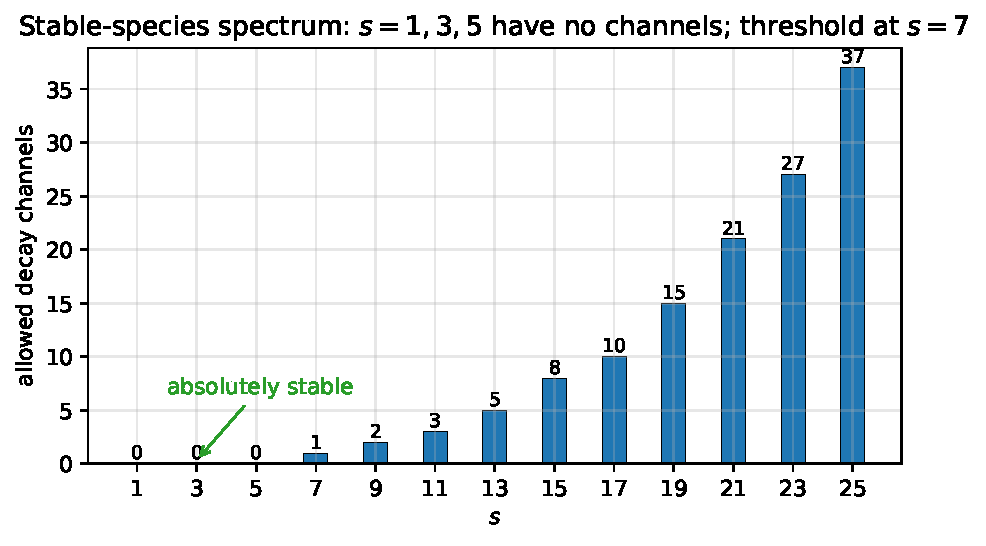
\includegraphics[keepaspectratio,alt={Figure 1. Stable-species spectrum and the decay threshold}]{figure_paper7_1_stable_species.pdf}}
\caption{Figure 1. Stable-species spectrum and the decay threshold}
\end{figure}

\textbf{Figure 1. Stable-species spectrum: the number of allowed decay
channels (odd partitions + capacity law, exhaustive). \(s=1,3,5\) have
zero channels (absolutely stable); the threshold is \(s=7\).}

\subsubsection{3.3 The terminal system}\label{the-terminal-system}

The final step of the cascade, \(3\to(1,1,1)\), is forbidden by
\(c(1)=1\). Hence \textbf{the all-1 state is unreachable}, and the
terminal population of the splitting cascade is a mixture of the stable
species \(\{1,3,5\}\). Moreover, the maximally dispersed configuration
within a single lattice is the one that ``fills one cell at a time from
the lowest shell'' (Fermi-sea type, \(n_{\max}\sim S^{2/3}\)).

\begin{center}\rule{0.5\linewidth}{0.5pt}\end{center}

\subsection{4. Timeless Branching
Ratios}\label{timeless-branching-ratios}

\subsubsection{4.1 Reformulating the
question}\label{reformulating-the-question}

If ``why does a stable state decay spontaneously'' is read as ``when,
and triggered by what,'' a background time flowing before the decay is
required. In this model time = a sequence of events (Paper 6), and there
is no time before an event. \textbf{The absence of a trigger =
spontaneity is an expression of the fact that time is constructed from
events.} The well-posed question decomposes into two: (i) which channels
are open (completed in §3), and (ii) what are the relative weights among
channels --- and (ii) is predictable by static counting.

\subsubsection{\texorpdfstring{4.2 The unique branching ratio at
\(s=9\)}{4.2 The unique branching ratio at s=9}}\label{the-unique-branching-ratio-at-s9}

The configuration counts of the two surviving channels (\(c(1)=1\),
\(c(3)=8\), \(c(5)=24\)):

\[
W(5,3,1)=24\times8\times1=192\;(77.4\%),\qquad
W(3,3,3)=\binom{8}{3}=56\;(22.6\%)
\]

\begin{quote}
Under equal weights on configurations (the counting principle), the
branching ratio is unique. The status of the equal-weight rule itself is
discussed in §8.
\end{quote}

\begin{figure}
\centering
\pandocbounded{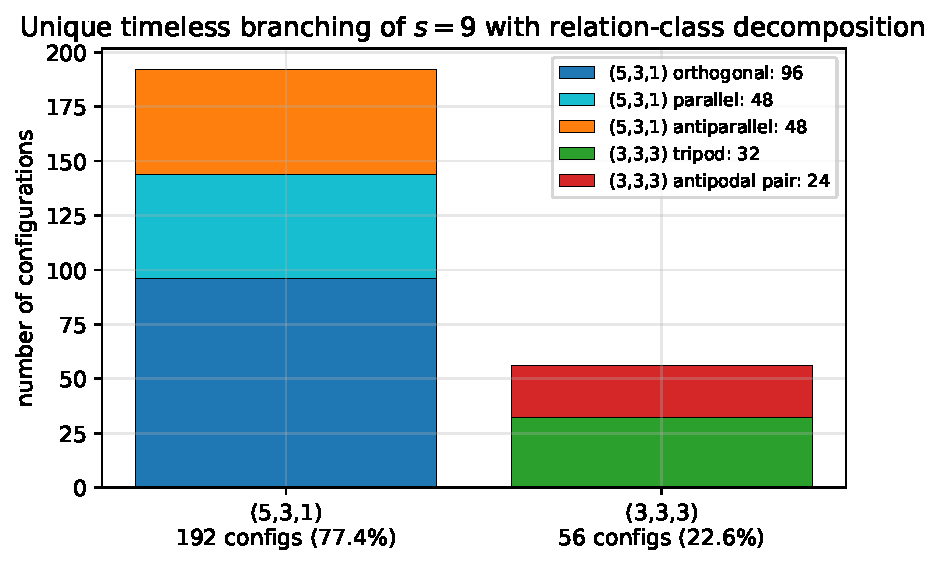
\includegraphics[keepaspectratio,alt={Figure 2. Unique timeless branching of s=9 with relation-class decomposition}]{figure_paper7_2_branching.pdf}}
\caption{Figure 2. Unique timeless branching of s=9 with relation-class
decomposition}
\end{figure}

\textbf{Figure 2. The unique timeless branching ratio of \(s=9\) (192:56
= 77.4\%:22.6\%) and the decomposition into the 5 relation classes
(breakdown of the 248 configurations).}

\subsubsection{4.3 The blocking effect (environment dependence of decay
channels)}\label{the-blocking-effect-environment-dependence-of-decay-channels}

In a shared lattice, existing occupancy blocks the channels of other
fragments. Example: in the fragment set \(\{7,3,1\}\), the unique
channel \((3,3,1)\) of \(7\) is \textbf{blocked} because the origin
(\(c(1)=1\)) is already occupied, so \(7\) is stabilized by its
environment. In \(\{9,3,1\}\), the \((5,3,1)\) channel of \(9\) is
blocked, and the branching ratio is modified by the environment to 100\%
\((3,3,3)\). \textbf{Stability and branching ratios are not attributes
of an isolated system but attributes of the configuration.}

\subsubsection{4.4 The state space as a finite closed
set}\label{the-state-space-as-a-finite-closed-set}

The reachable configurations for small \(S\) can be enumerated
completely (example: \(S_0=9\) gives the 3 configurations
\(\{9\},\{5,3,1\},\{3,3,3\}\), with \(1+3+2=6\) gauge-invariant states).
That the timeless state space can be held in one's hand as a finite
transition system is the core of the verifiability of this model.

\begin{center}\rule{0.5\linewidth}{0.5pt}\end{center}

\subsection{5. The Birth of Relational
Geometry}\label{the-birth-of-relational-geometry}

The configuration of a single fragment (its position on a shell) is a
purely non-observable under the \(B_4\) gauge (Paper 6 §4). Since
\(B_4\subset O(4)\) preserves inner products, \textbf{with two or more
fragments, for the first time, the inner products = angles between
occupied cells become observable as gauge invariants.}

The 248 final decay configurations of \(s=9\) (\((5,3,1)\): 192,
\((3,3,3)\): 56) split into 5 relation classes under the \(B_4\) orbit
decomposition:

{\def\LTcaptype{none} % do not increment counter
\begin{longtable}[]{@{}
  >{\raggedright\arraybackslash}p{(\linewidth - 6\tabcolsep) * \real{0.2143}}
  >{\raggedright\arraybackslash}p{(\linewidth - 6\tabcolsep) * \real{0.2143}}
  >{\raggedleft\arraybackslash}p{(\linewidth - 6\tabcolsep) * \real{0.2857}}
  >{\raggedleft\arraybackslash}p{(\linewidth - 6\tabcolsep) * \real{0.2857}}@{}}
\toprule\noalign{}
\begin{minipage}[b]{\linewidth}\raggedright
Class
\end{minipage} & \begin{minipage}[b]{\linewidth}\raggedright
Invariant
\end{minipage} & \begin{minipage}[b]{\linewidth}\raggedleft
Configurations
\end{minipage} & \begin{minipage}[b]{\linewidth}\raggedleft
Fraction
\end{minipage} \\
\midrule\noalign{}
\endhead
\bottomrule\noalign{}
\endlastfoot
\((5,3,1)\) orthogonal type & \(\langle v_5,v_3\rangle=0\) & 96 &
38.7\% \\
\((5,3,1)\) parallel type & \(+1\) & 48 & 19.4\% \\
\((5,3,1)\) antiparallel type & \(-1\) & 48 & 19.4\% \\
\((3,3,3)\) tripod type & 3 mutually orthogonal axes & 32 & 12.9\% \\
\((3,3,3)\) antipodal-pair type & contains an antipodal pair & 24 &
9.7\% \\
\end{longtable}
}

A single fragment has no position; \textbf{the relative structure of the
configuration is the first intrinsic geometric observable.}

\begin{center}\rule{0.5\linewidth}{0.5pt}\end{center}

\subsection{\texorpdfstring{6. \(\lambda\)-Side Readout: Holographic
Identification of the Relation
Classes}{6. \textbackslash lambda-Side Readout: Holographic Identification of the Relation Classes}}\label{lambda-side-readout-holographic-identification-of-the-relation-classes}

\subsubsection{6.1 The readout model and the structure of the
record}\label{the-readout-model-and-the-structure-of-the-record}

By the record theorem (Paper 6), every observable must be readable as a
\(\lambda\)-side record. To each occupied cell we associate the real
standing wave \(\Phi_k\) of the dictionary (Paper 5), and take as the
\(\lambda\)-side record of a configuration the intensity
\(I(x)=\Psi(x)^2\), \(\Psi=\sum_{k}\Phi_k\). By the product-to-sum
formula, \textbf{the \(\lambda\)-side record = the autocorrelation
spectrum of the configuration}, and the cross terms lie on the pairwise
sum and difference vectors of the occupied cells.

\subsubsection{6.2 Complete separation of the 5 classes (a theorem over
all 248
configurations)}\label{complete-separation-of-the-5-classes-a-theorem-over-all-248-configurations}

The (norm²: line count) data of the multiplicity- and amplitude-weighted
power spectrum alone completely separates the 5 classes: orthogonal
\((1{:}1,\,3{:}4)\), parallel \((1{:}2,\,5{:}2)\), antiparallel
\((1{:}1,\,5{:}2)\), tripod \((2{:}6)\), antipodal-pair \((2{:}4)\). The
peak intensities (\(19.49/19.49/11.90/18/11.66\)) are an independent
consistency check. By closed forms independent of the choice of branch,
axis, and sign, \textbf{within-class constancy over all 248
configurations} holds as a theorem.

\begin{figure}
\centering
\pandocbounded{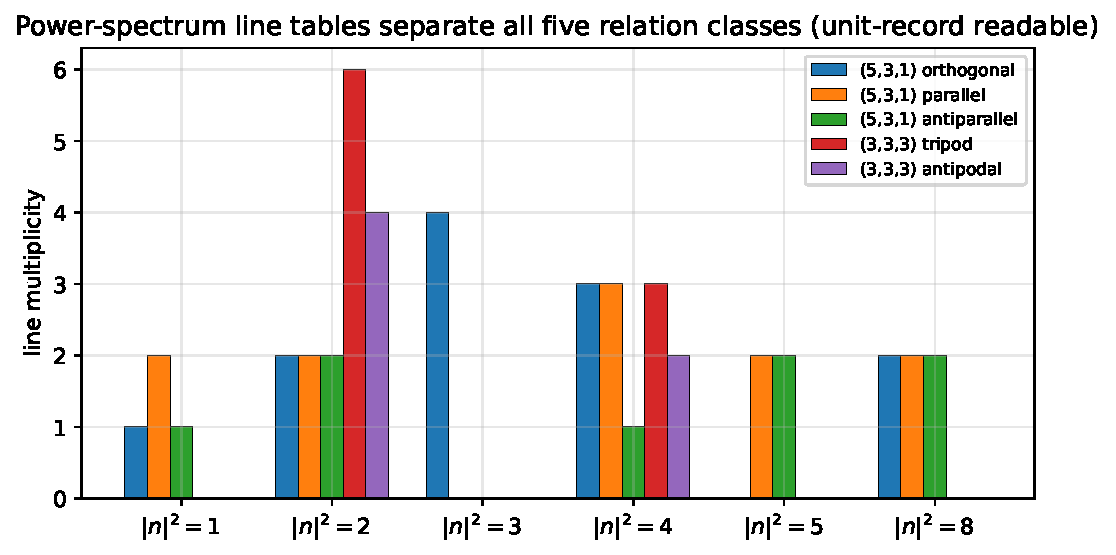
\includegraphics[keepaspectratio,alt={Figure 3. Complete line tables of the five relation classes}]{figure_paper7_3_line_tables.pdf}}
\caption{Figure 3. Complete line tables of the five relation classes}
\end{figure}

\textbf{Figure 3. Complete line tables of the 5 relation classes:
complete separation by the multiplicity-weighted power spectrum (norm²:
line count) alone --- all the data readable from a single unit record.}

\subsubsection{6.3 The unit-record sufficiency
theorem}\label{the-unit-record-sufficiency-theorem}

The spectral lines of the interference intensity --- cross terms and
self terms alike --- lie on integer frequency vectors, and integer
frequency modes are exactly orthogonal on the unit cell. Therefore:

\begin{quote}
\textbf{From the \(\lambda\) record of a single unit cell, the
amplitudes of all spectral lines can be determined exactly.} What is
needed is not super-resolution but exactly the resolution of the unit
record.
\end{quote}

Since \(I(x)\) is a trigonometric polynomial of degree \(\le 2\) per
axis, it can be reconstructed exactly from a lattice sample of 5 equally
spaced points per axis, \(5^4=625\) points in total (a finite,
constructive readout procedure).

\subsubsection{6.4 The digital amplitude
alphabet}\label{the-digital-amplitude-alphabet}

The amplitudes of all lines lie on the discrete set
\(\{\tfrac12,1,\sqrt2,2,2\sqrt2\}=(\sqrt2)^j\). The readout is
\textbf{digital decoding}, for which a relative precision of about ±20\%
suffices.

\subsubsection{6.5 Holographic type and interferometric
type}\label{holographic-type-and-interferometric-type}

A line of amplitude \(2\sqrt2\) is \(2\Phi_0\Phi_k=2\Phi_k\), i.e., a
linear transcription of a component wave, and it appears only when an
\(s=1\) fragment (the zero mode = the constant wave) is present.

\begin{itemize}
\tightlist
\item
  \textbf{\((5,3,1)\) type (with reference) = holographic}: from the
  linear transcription, the configuration can be completely
  reconstructed down to the cell and branch of each fragment. This is
  the same structure as Gabor's holography with a reference beam
  {[}10{]} (a structural correspondence, not an identification).
\item
  \textbf{\((3,3,3)\) type (no reference) = interferometric}: only the
  pairwise relations can be read.
\end{itemize}

The presence or absence of the minimal fragment divides the
\textbf{information class} of the record. Moreover, the DC component of
the intensity equals the fragment number \(n\), so the count and the
\(Z_2\) parity are directly readable on the \(\lambda\) side.

\begin{center}\rule{0.5\linewidth}{0.5pt}\end{center}

\subsection{7. Scope of Claims of This
Paper}\label{scope-of-claims-of-this-paper}

What this paper claims: (1) The derivation of exclusion statistics from
the configuration reading. (2) The shell capacity law, the stable
species \(\{1,3,5\}\), and the threshold \(s=7\) (exhaustive scan). (3)
The unique branching ratio at \(s=9\) (under equal weights). (4) The
blocking effect and the finite closed state space. (5) The complete
\(\lambda\)-side readout of the relation classes (the theorem over all
248 configurations, unit-record sufficiency, the digital alphabet, and
the two information classes).

What this paper does not claim: (1) Identification with physical
particles or matter fields (``exclusion,'' ``statistics,'' and
``branching ratio'' are descriptions of counting structures within the
model). (2) Absolute values of transition rates or lifetimes (dynamics
is out of scope; predictions are limited to ratios). (3) A
first-principles derivation of the equal-weight rule (§8). (4) Exclusion
of embeddings other than the configuration reading (the readout theorems
constitute passing an independent test of the configuration reading, not
a proof of uniqueness).

\begin{center}\rule{0.5\linewidth}{0.5pt}\end{center}

\subsection{8. Discussion}\label{discussion}

\textbf{The status of the equal-weight rule.} In standard statistical
mechanics the equal a priori probability is a postulate {[}8{]}. In this
model, equal weights on allowed configurations are the expression of
minimality --- ``introduce no weighting principle other than counting''
--- and in a subsequent paper we will show that no weight other than
configuration counting is generated by the kinematics (an impossibility
theorem for weight derivation).

\textbf{Observability of relations only.} The constraint that ``only
relative quantities are meaningful,'' discussed in a general framework
by the theory of reference frames {[}9{]}, is realized in this model
from the record theorem + the \(B_4\) gauge, complete with a concrete
readout procedure (§6). In particular, the mechanism by which the
presence or absence of a reference (the zero mode) switches the class of
readable information reproduces, inside a counting model, the structure
of holography and heterodyne detection.

\textbf{The origin of the statistics.} The Pauli exclusion principle
{[}5{]} has been reduced in this model to ``being a set +
orthogonality.'' This is not an explanation of physical fermions, but it
provides one example of ``what minimal structure can generate
exclusion.''

\begin{center}\rule{0.5\linewidth}{0.5pt}\end{center}

\subsection{9. Conclusion}\label{conclusion}

From the minimal embedding hypothesis of the configuration reading,
exclusion statistics, the stable-species spectrum, the unique timeless
branching ratio, and the blocking effect have been derived; relational
geometry (angles) is born; and it has been established as a theorem that
all of its information can be read out by digital decoding of a unit
record. In particular, the exact match --- ``the resolution required for
identification = the resolution of the unit record,'' with nothing to
spare and nothing lacking --- is independent evidence that the
configuration reading is consistent with the record structure.

Paper 8 will construct on top of these statistics the two accountings
(condensation and expansion), and Paper 9 the wave-theoretic derivation
of the stability of composites.

\begin{center}\rule{0.5\linewidth}{0.5pt}\end{center}

\subsection{Appendix: Essentials of the Reproduction
Procedure}\label{appendix-essentials-of-the-reproduction-procedure}

The stable-species scan is the full enumeration of odd partitions + the
capacity filter (\(s\le25\)); the branching ratios come from direct
enumeration of shell cells (\(c(1),c(3),c(5)=1,8,24\)); the relation
classes come from canonicalization under \(B_4\) (384 elements) and
orbit counting (verification of \(96+48+48+32+24=248\)); the readout
rests on the closed forms of the product-to-sum expansion and numerical
cross-checking. The scripts and research notes are provided in the
public repository (https://github.com/WurabeSeiji/ai-chat-logs-open).

\begin{center}\rule{0.5\linewidth}{0.5pt}\end{center}

\subsection{References}\label{references}

{[}1{]} Noriaki Kihara, Paper 4, v1.0, 2026. Concept DOI:
10.5281/zenodo.20638962.

{[}2{]} Noriaki Kihara, Paper 5, v0.2, 2026. Concept DOI:
10.5281/zenodo.20640454.

{[}3{]} Noriaki Kihara, Paper 6, v0.2, 2026. Concept DOI:
10.5281/zenodo.20640456.

{[}4{]} Noriaki Kihara, Paper 2, v0.2, 2026. Concept DOI:
10.5281/zenodo.20588038.

{[}5{]} W. Pauli, ``Über den Zusammenhang des Abschlusses der
Elektronengruppen im Atom mit der Komplexstruktur der Spektren,''
Zeitschrift für Physik 31 (1925), 765--783.

{[}6{]} E. Fermi, ``Zur Quantelung des idealen einatomigen Gases,''
Zeitschrift für Physik 36 (1926), 902--912.

{[}7{]} P. A. M. Dirac, ``On the theory of quantum mechanics,''
Proceedings of the Royal Society A 112 (1926), 661--677.

{[}8{]} E. T. Jaynes, ``Information theory and statistical mechanics,''
Physical Review 106 (1957), 620--630.

{[}9{]} S. D. Bartlett, T. Rudolph, and R. W. Spekkens, ``Reference
frames, superselection rules, and quantum information,'' Reviews of
Modern Physics 79 (2007), 555--609.

{[}10{]} D. Gabor, ``A new microscopic principle,'' Nature 161 (1948),
777--778.

\begin{center}\rule{0.5\linewidth}{0.5pt}\end{center}

\subsection{License}\label{license}

This paper is published under CC BY 4.0.\\
Reuse, adaptation, translation, and citation are permitted, provided
that the author name, version, publication date, and source are clearly
indicated.

\end{document}
